%# -*- coding: utf-8-unix -*-
% !TEX program = xelatex
% !TEX root = ../thesis.tex
% !TEX encoding = UTF-8 Unicode
%%==================================================
%% chap3compare.tex for SJTU Master Thesis
%%==================================================

%\bibliographystyle{sjtu2}%[此处用于每章都生产参考文献]
\chapter{儿科肠道炎症性疾病与肠道菌群研究}
\label{chap:compare}

\section{引言}
坏死性小肠结肠炎(Necrotizing Enterocolitis,NEC)、先天性巨结肠小肠结肠炎(Hirchsprung-Associated Enterocolitis )和炎症性肠病(Inflammatory Bowel Disease,IBD)为常见的儿科肠道炎症性疾病\cite{neu2011necrotizing,levine2014espghan,frykman2012hirschsprung}。尽管发病年龄不尽相同,但它们有着相似的临床表现(腹痛、呕吐、腹泻、便秘、血便、喂养不耐受、体重减轻甚至营养不良)和病理改变(小肠、结肠肠粘膜损伤、坏死、固有层局部中性粒细胞浸润等)\cite{yu1980improving}。以往研究表明,幼时罹患HAEC的患儿日后患IBD的风险增加,且免疫介导的炎症性疾病患者肠道菌群具有相似性。那么,肠道菌群在上述疾病中的改变是否是其相似的临床和病理特点的因素之一?监控患儿早期肠道菌群异常并及时优化、干预是否有助于降低日后罹患IBD的风险?本研究旨在对上述肠道炎症性疾病病程中的菌群特征进行初步探索,致力寻找其共有的生物标记物,为其防治提供依据。

\section{材料与方法}
  \subsection{伦理}
  该研究经上海市儿童医学中心伦理联合委员会批准,上海交通大学医学院(SCMCIRB-K2013022)。 在采集每名患儿的粪便样本之前,取得其监护人理解、同意并于知情同意书上签字。
  \subsection{研究对象}
  于2017年3月至2018年6月间,上海儿童医学中心新生儿重症监护病房(NICU)的NEC患儿、外科病房的HD、HAEC患儿和上海市儿童医院消化科病房的IBD患儿,
    \subsubsection{NEC入选及排除标准}
      \paragraph{入组标准}
      胎龄小于34周,出生体重不低于950g的住院患儿。
      \paragraph{排除标准}
      1)新生儿早发型脓毒血症,2)肝脏疾病,3)肾功能损害(Cr>88μM),4)存在先天肠道发育异常,5)需要进行大型胸部或腹部手术(男性包皮环切术或动脉导管结扎除外),6)预计使用肠外营养(Parental Nutrition, PN)支持供应超过50%的每日卡路里摄入量,且时间超过4天,7)静脉注射抗生素(除头孢噻肟、哌拉西他唑和甲硝唑),8)有口服抗生素史,9)有血便史,10)日龄大于五天者
    \subsection{HD和HAEC入选及排除标准}
      \paragraph{入选标准} 1)病理确诊HD的患儿和确诊的HAEC患儿;2)需要接受手术治疗HD的患儿;3)年龄0~4岁。
      \paragraph{排除标准} 1)合并其它疾病或畸形(如先天性心脏病、唐氏综合症等),2)入组前一周内接受过抗生素,3)入组前三个月内接受过益生菌制剂。
    \subsection{IBD入选及排除标准}
      \paragraph{入选标准} 根据儿童和青少年炎症性肠病的诊断标准指南\cite{levine2014espghan},初次诊断儿童克罗恩病和溃疡性结肠炎的患儿。
      \paragraph{排除标准} 曾经接受过肠切除手术的患儿。
  \subsection{诊断标准}
    坏死性小肠结肠炎(NEC)诊断和分级:关注每名患儿入院后的健康情况,评估并记录一般情况全身,腹部平片报告结果等;根据“改良Bell分级标准”\cite{bell1978neonatal}:II期,伴有放射性肠扩张,肠梗阻,肠道积气和/或腹部压痛,和/或轻度代谢性酸中毒,肠鸣音减弱,血小板减少症。

    先天性巨结肠(HD)诊断标准为Elhalaby临床诊断标准\cite{elhalaby1995enterocolitis}和Teitelbaum病理诊断标准。

    先天性巨结肠小肠结肠炎诊断标准依据美国儿科协会的临床诊断标准\cite{imamura1992mucosal}:基于病史、临床症状(呕吐、腹胀)以及影像学表现(腹部平片可见积气或液平等)。

    炎症性肠病(IBD)的准确诊断:基于病史,体格检查和实验室检查,食管胃十二指肠镜检查(EGD)和组织学的回肠结肠镜检查以及小肠镜的组合。



  \subsection{主要实验室试剂及仪器}
  参照\ref{主要实验室试剂及仪器}
  \subsection{粪便标本采集方法}
  参照\ref{粪便标本采集方法}
  \subsection{标本总DNA提取}
  参照\ref{标本总DNA提取}
  \subsection{总DNA 16s rRNA V3-V4可变区片段的扩增}
  参照\ref{总DNA 16s rRNA V3-V4可变区片段的扩增}
  \subsection{荧光定量}
  参照\ref{荧光定量}
  \subsection{Illumina Miseq下一代高通量测序}
  参照\ref{Illumina Miseq下一代高通量测序}
  \subsection{原始数据处理}
  参照\ref{原始数据处理}
  \subsection{统计学方法}
  参照\ref{统计学方法}
  \begin{enumerate}
    \item 使用KW test和卡方检验比较患者临床基本信息。
    \item 使用Kruskal-Wallis H test检验各分类水平下各物种在各组间的分布(相对丰度)是否存在显著性差异;使用Benjaminia and Hochberg法对\textit{p}值进行多重检验矫正。使用Student’s \textit{t}检验检验各分类水平下各物种在两个组之间的分布(相对丰度)是否存在显著性差异;使用Benjaminia and Hochberg法对\textit{p}值进行多重检验矫正。
    \item 使用Student’s t检验评估两组间多样性指数的差异。若p < 0.05 则表示差异有统计学意义。通过$\alpha$多样性分析可以得到群落(分组或者单个样本)中物种的丰度、覆盖度和多样性等信息。
    \item 利用Wilcoxon秩和检验,对每一组中的亚组进行两两检验,在具有显著差异物种类中的所有亚种比较是否都趋同于同一分类级别。
  \end{enumerate}

\section{结果}
  \subsection{患者基本情况及样本测序信息}
  入选HAEC患儿4例,HD患儿7例,NEC患儿6例,IBD患儿7例,共24例。采集其横向粪便标本,共58个,其中HAEC标本14个,HD标本22个,NEC标本15个,IBD标本7个。其他临床资料见表\ref{tab:comparedemographic}。

  \begin{table}[!hpb]
    \centering
    \bicaption[HAEC,HD,NEC,IBD患者临床情况]
      {HAEC,HD,NEC,IBD患者临床情况}
      {Demographic characteristics of HAEC, HD, NEC, and IBD groups.}
    \label{tab:comparedemographic}
    \begin{tabular}{lp{1.8cm}p{1.6cm}p{1.8cm}p{1.8cm}p{2cm}c}
      \toprule
         & \textbf{HAEC (N=4)} & \textbf{HD (N=7)} & \textbf{NEC (N=6)} & \textbf{IBD (N=7)} & \textbf{Statistical Test} & \textit{p value} \\ \midrule
        \textbf{年龄(天)} & 415(147-1162) & 214(79-368) & 115(62-220) & 3451(372-5110) & Kruskal-Wallis test & < 0.01 \\
        \textbf{胎龄(周)} & 36(33-37) & 38(37-41) & 33(29-37) & 37(37-37) & Kruskal-Wallis test & 0.111 \\
        \textbf{住院时间(天)} & 11(4-15) & 17(10-29) & 46(10-95) & NA & Kruskal-Wallis test & 0.365 \\
        \textbf{性别} &  &  &  & & Fisher's test & 0.628 \\
        \multicolumn{1}{r}{女} & 1(25\%) & 1(14\%) & 2(33\%) & 2(29\%) &  & \\
        \multicolumn{1}{r}{男} & 3(75\%) & 6(86\%) & 4(67\%) & 5(71\%) &  &\\
         \bottomrule
    \end{tabular}
  \end{table}

  使用Illumina MiSeq高通量测序、优化后,得到2,749,518条16s rRNA gene reads,优化碱基数目共1223776595,优化平均序列长度为445bp。

  \subsection{多样性分析}
    \subsubsection{$alpha$多样性分析}
    基于OTU进行计算,HAEC,HD,NEC,IBD组shannon多样性指数分别为1.69、1.75、1.44、2.08:,两两比较未见明显统计学差异(HAEC vs HD p = 0.34;HAEC vs NEC p = 0.79;HAEC vs IBD p = 0.08;HD vs NEC p = 0.35;HD vs IBD p = 0.31;NEC vs IBD p = 0.07)(图\ref{fig:3alphadiversity:shannon});HAEC,HD,NEC,IBD组simpson指数分别为0.41、0.34、0.36、0.24:两两比较未见明显统计学差异(HAEC vs HD p = 0.47;HAEC vs NEC p = ;HAEC vs IBD p = 0.18;HD vs NEC p = 0.57;NEC vs IBD p = 0.15)(图\ref{fig:3alphadiversity:simpson})。
      %alpha多样性图
      \begin{figure}[!htp]
        \centering
          \subcaptionbox{Shannon指数\label{fig:3alphadiversity:shannon}}
            {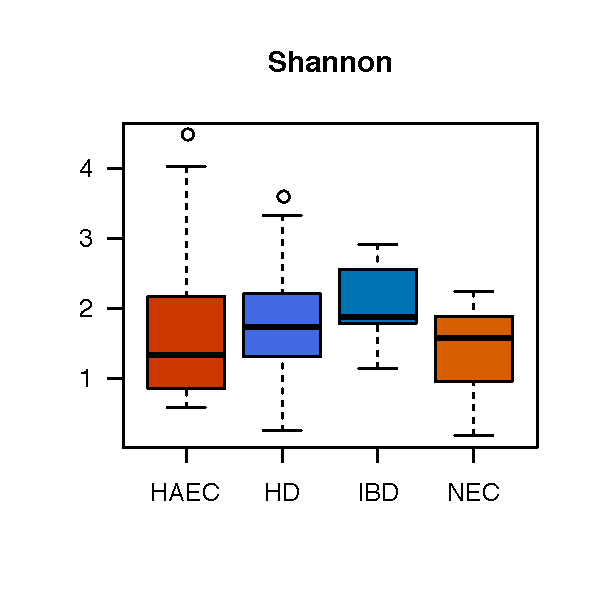
\includegraphics[height=5.5cm]{figure/3shannon.pdf}}
            \hspace{4em}
          \subcaptionbox{Simpson指数\label{fig:3alphadiversity:simpson}}
            {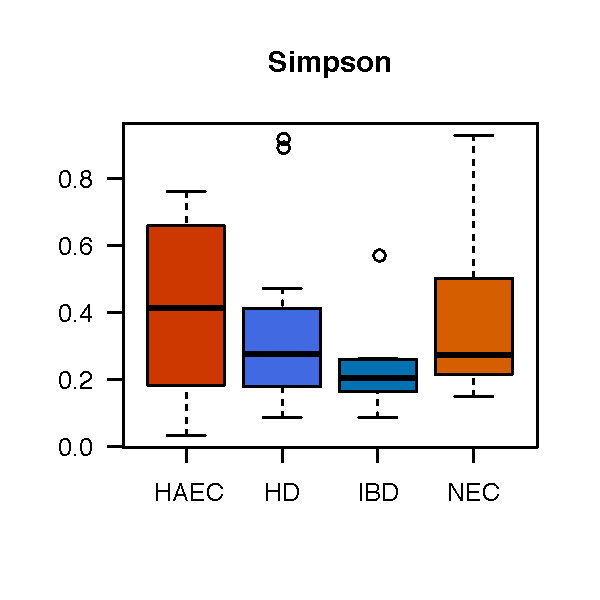
\includegraphics[height=5.5cm]{figure/3simpson.pdf}}
        \bicaption[HAEC,HD,NEC和IBD患儿间肠道菌群$\alpha$多样性比较]{通过计算Shannon指数(a)和Simpson(b)指数对HAEC,HD,NEC,IBD患儿间肠道菌群$\alpha$多样性分析}{Exploring $\alpha$ diversity by calculation Shannon diversity index(a) and Simpson diversity index(b) among preterm infants with HAEC,HD,NEC and IBD groups.}
        \label{fig:3alphadiversity}
      \end{figure}

    \subsubsection{$beta$多样性分析}
    使用基于bray-curtis距离的主坐标(PCoA)进行分析发现,四组患儿肠道菌群在菌群整体结构上未见明显差异,PC1 = 32.07\%, PC2 = 24.84\%(图\ref{fig:3beta})。
      \begin{figure}[!htp]
        \centering
        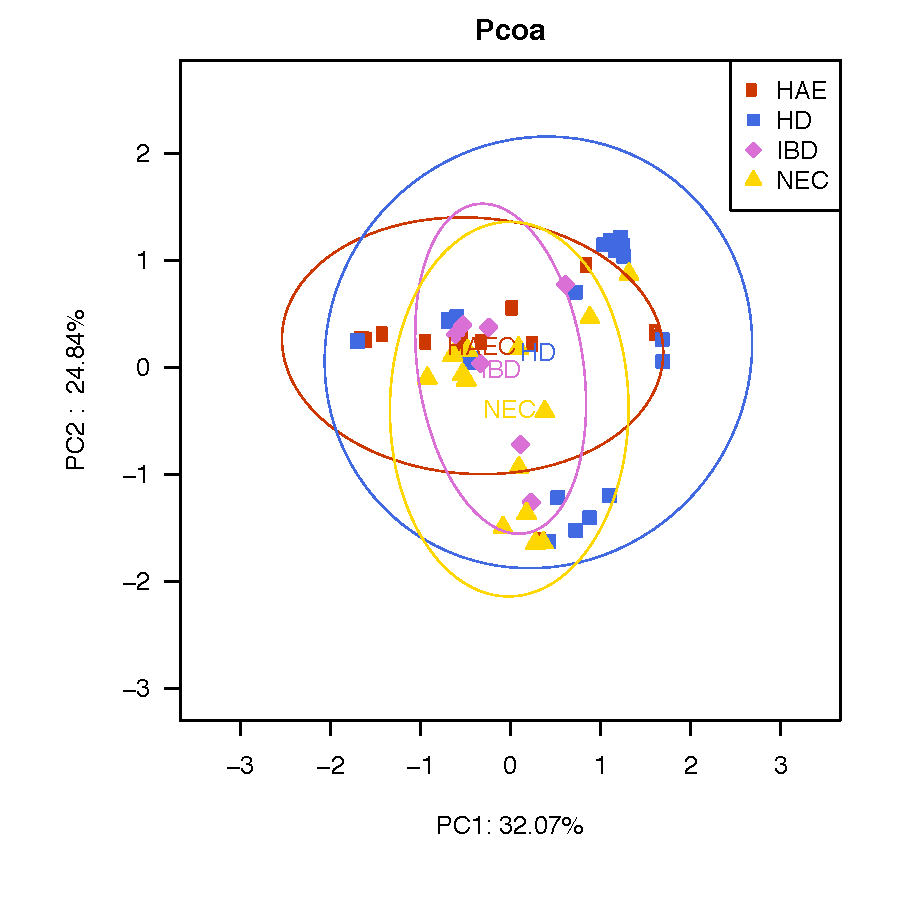
\includegraphics[width=15cm]{3beta.pdf}
        \bicaption[四组患儿肠道菌群整体结构对比]
          {使用bray-curtis距离对四组患儿肠道菌群进行PCoA分析}
          {Colonization Pattern among HAEC, HD, NEC, and IBD groups by PCoA of Bray-Curtis Distances}
        \label{fig:3beta}
      \end{figure}

  \subsection{分类学分析}
  对于测序数据进行OTU聚类,采用RDP classifier贝叶斯算法对97\%相似水平的OTU代表序列进行分类学分析,并分别在各个分类水平(从域(domain)到属(genus))统计各样本的群落组成,比对silva数据库得出各群落数量。
    \subsubsection{门(phylum)水平}
    在门水平,四组患儿肠道内以变形菌门(\textit{Proteobacteria})、厚壁菌门(\textit{Firmicutes})、拟杆菌门({\textit{Bacteroidetes})和放线菌门({\textit{Actinobacteria})为主导。HAEC和IBD组有着类似的菌群组成,而HD和NEC组菌群组成则类似。HAEC和IBD组厚壁菌门和变形菌门丰度相仿(厚壁菌门HAEC 53.15\%,HD 59.84\%,p = 0.78;变形菌门HAEC 24.01\%,HD23.96 \%, p = 0.87)(图\ref{fig:3phylum})。另外, \textit{Verucomicobia}(1.67\%)和\textit{Synergistetes}(1.37\%)菌门为HAEC所独有。
      %门水平配图
      \begin{figure}[!htp]
        \centering
        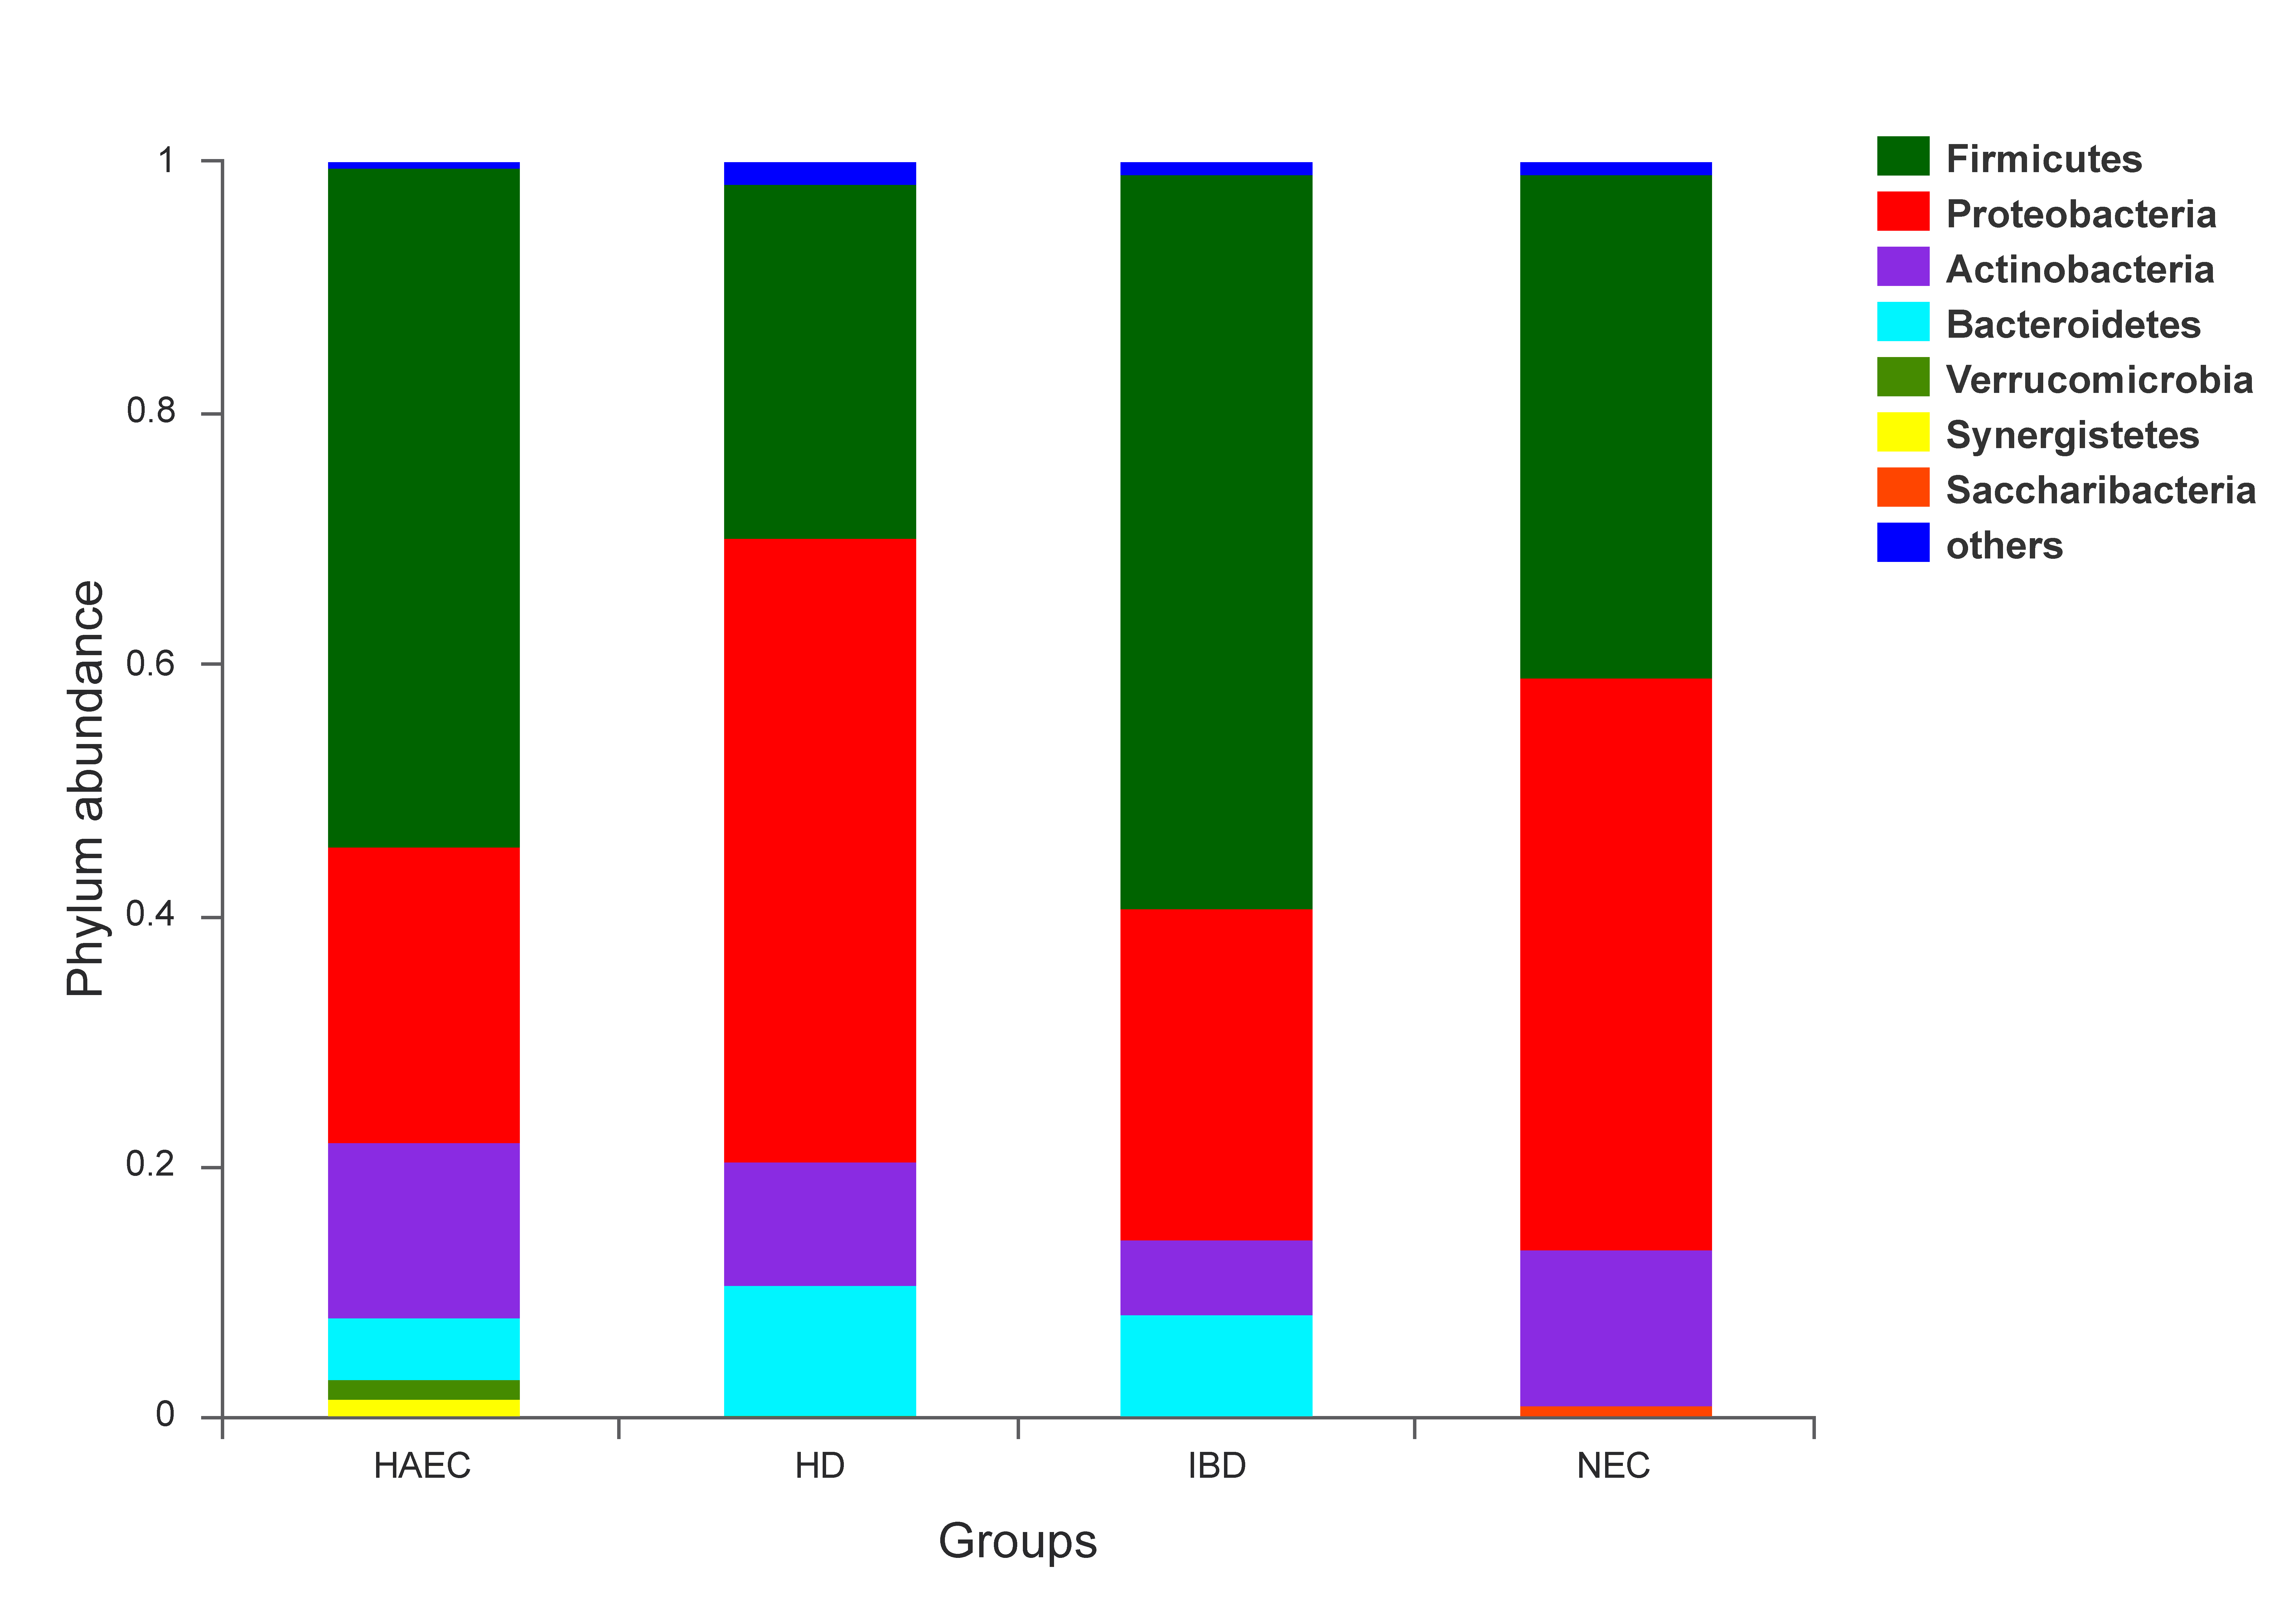
\includegraphics[width=15cm]{3phylum.pdf}
        \bicaption[门水平上HAEC, HD, NEC, 和IBD患儿菌群相对丰度]
          {门水平上HAEC, HD, NEC, 和IBD患儿菌群相对丰度。}
          {Relative Abundance of Phylum in Intestinal Microbiota.}
        \label{fig:3phylum}
      \end{figure}

    \subsubsection{属(genus)水平}
    在属水平上,HAEC组患儿肠道以肠球菌属(\textit{Enterococcus})为主导(38.02\%),且丰度远高于另三组(HD 16.06\%,NEC 5.86\%,IBD14.98\%,p = 0.01);HD组以埃希菌-志贺菌属(\textit{Escherichia-Shigella})占主导,丰度达26.04\%,与其余三组差异不显著(p = 0.06);IBD组以韦荣球菌属(\textit{Veillonella})为优势菌群(14.00\%),且显著高于其余三组(p = 0.02);NEC菌群组成较前三组则更为简单,以克雷伯菌属(\textit{Klebsiella})为主,丰度为25.14\%,与其余三组丰度未见显著差异(p = 0.25)(图\ref{fig:3genus})。
      %属水平配图
      \begin{figure}[!htp]
        \centering
        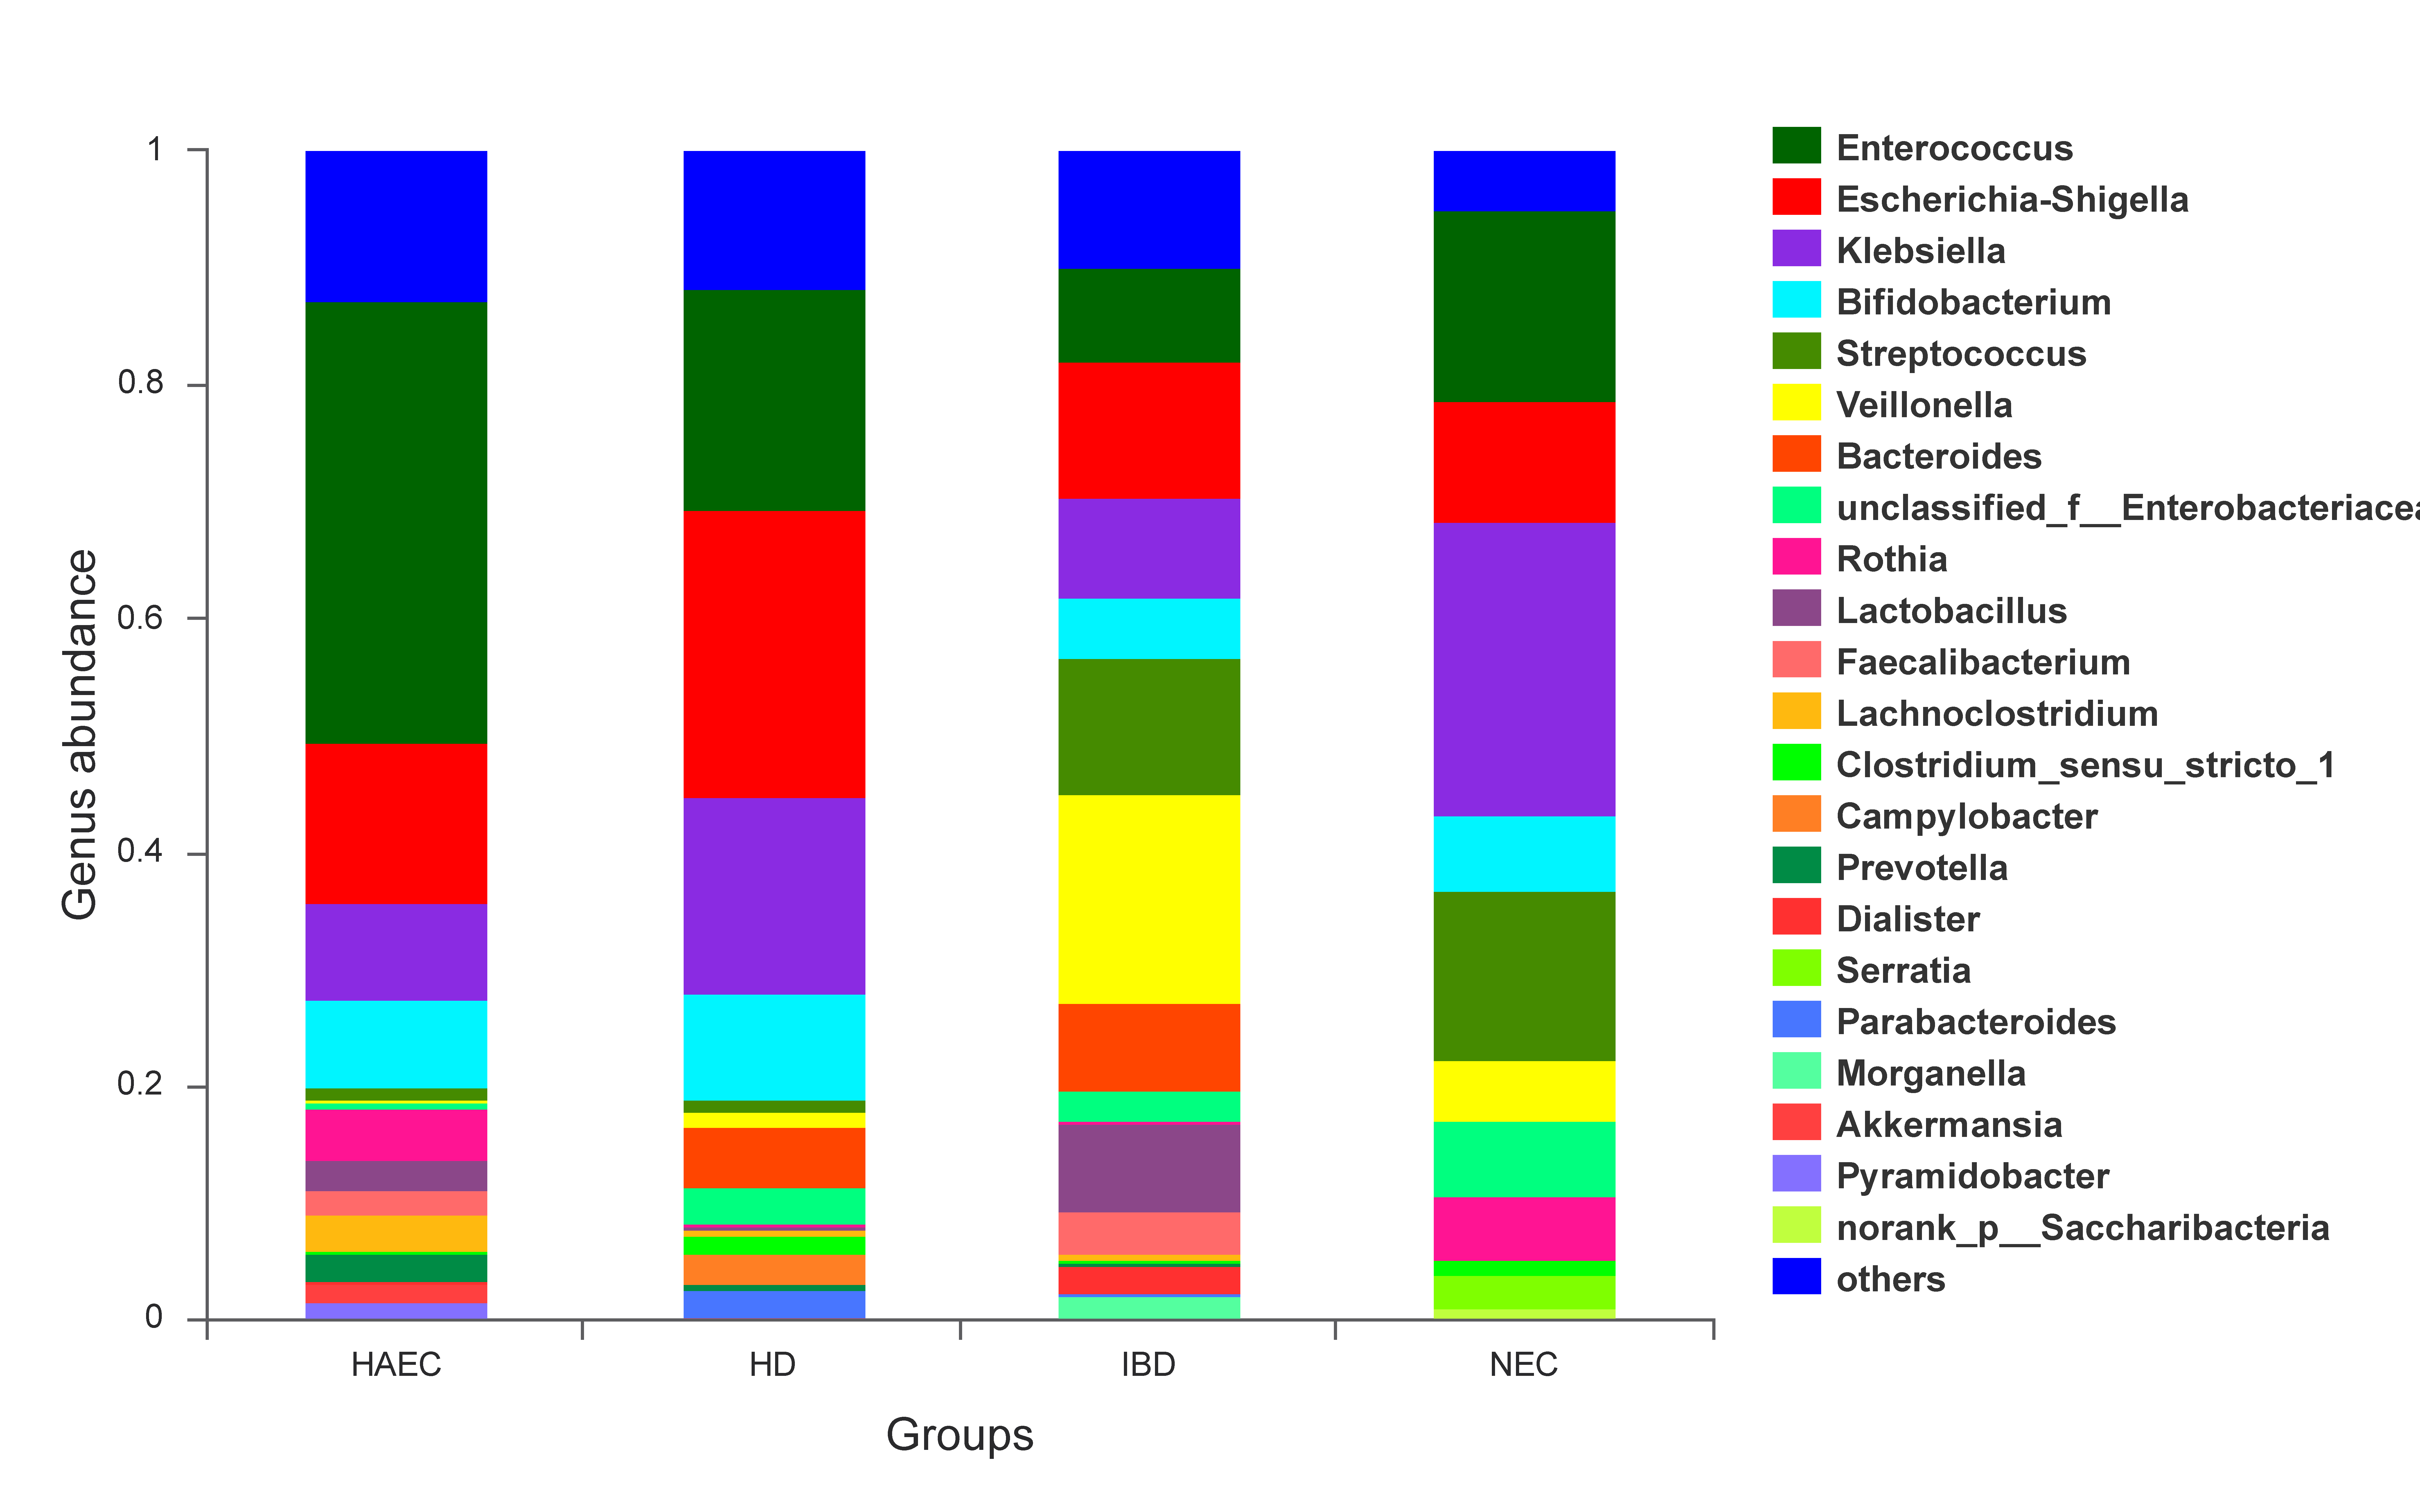
\includegraphics[width=15cm]{3genus.pdf}
        \bicaption[属水平上HAEC, HD, NEC, 和IBD患儿菌群相对丰度]
          {属水平上HAEC, HD, NEC, 和IBD患儿菌群相对丰度。}
          {Relative Abundance of Genus in Intestinal Microbiota.}
        \label{fig:3genus}
      \end{figure}

    \subsubsection{多级物种差异判别分析(LEfSe分析)}
    通过LEfSe分析结果显示,HAEC、NEC和IBD组在菌群在分类进化上具有较大的吻合,具体包括厚壁菌门(\textit{Firmicutes})(LDA = 5.27)、芽孢杆菌纲(\textit{Bacillus})(LDA = 5.07)、\textit{Negativicutes}菌纲(LDA = 4.97)、\textit{Selenomonadales}菌目(LDA = 4.97)和乳杆菌目(\textit{Lactobacillales})(LDA = 5.07)和肠球菌属(\textit{Enterococcus})(LDA = 5.20);而HD组则以拟杆菌门\textit{Bacteroidetes}及其分支菌属为代表(LDA = 4.76)。
    %LDA配图
    \begin{figure}[!htp]
      \centering
      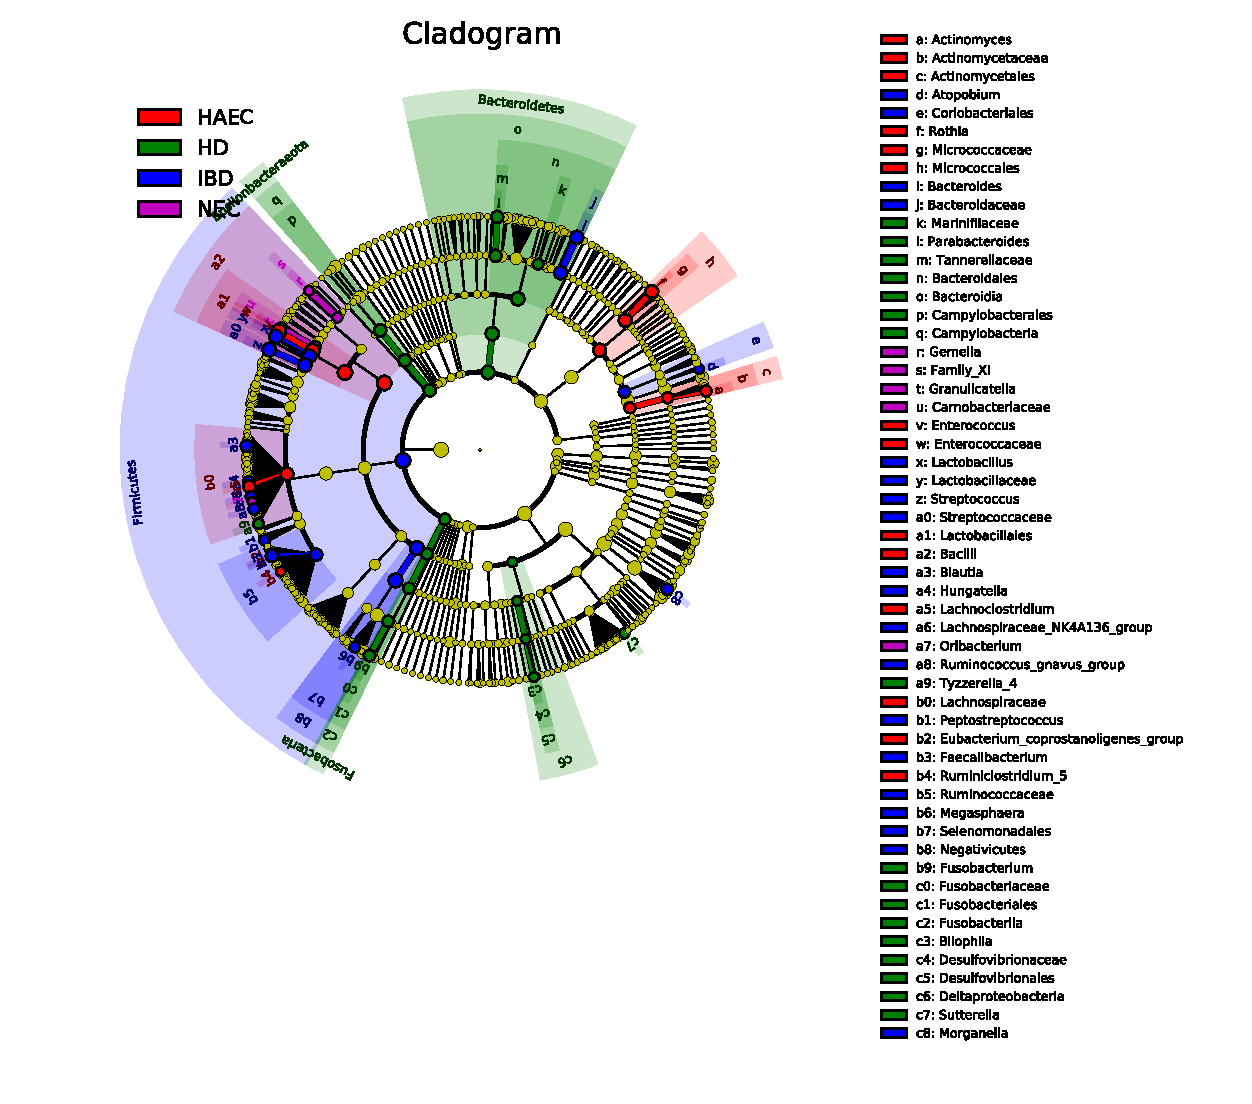
\includegraphics[width=15cm]{3clado.pdf}
      \bicaption[LEfSe分析HAEC, HD, NEC, 和IBD患儿菌群]
        {HAEC, HD, NEC, 和IBD患儿菌群LEfSe进化分支图。红色代表HAEC组,绿色代表HD组,蓝色代表IBD组,紫色代表NEC组。}
        {Cladogram generated by software LEfSe. The red part represents the HAEC group. The green part represents the HD group. The blue part represents the IBD group and the purple one represents the NEC group. }
      \label{fig:3clado}
    \end{figure}
\section{讨论}
  先天性巨结肠小肠结肠炎(HAEC)、坏死性小肠结肠炎(NEC)和炎症性肠病(IBD)均为儿科常见的肠道炎症性疾病,其发病与遗传、环境因素、肠道免疫功能相关\cite{Downard2012Treatment, Santha2017Mucosal, Denning2016Pathogenesis}。 近年来,各腔道微生物成为儿科肠道炎症性疾病病因学研究的热点。其中,肠道黏膜免疫和肠道菌群失调在其发生发展中的作用及机制研究不断深入。16S rRNA 高通量测序技术的广泛应用使得肠道微生物群得以更全面对分析。

  在临床实践中,我们观察到,三种肠炎的患儿都有着类似的临床症状,包括腹痛、腹胀、血便、喂养不耐受,严重者甚至危及生命;其病理表现亦有相似之处,包括小肠、结肠肠粘膜损伤、坏死、固有层局部中性粒细胞浸润等。既往研究表明,肠道菌群紊乱均见于此三种疾病,具体来说,IBD的发生常常伴随着厚壁菌门(\textit{Firmicutes})丰度的升高,NEC发病与肠道变形菌门(\textit{Proteobacteria})丰度升高相关\cite{Hosny2017Updating},而HAEC患儿肠道内则独有韦荣球菌\cite{Yan2014Characterization,Li2016Characterization}。另外,有meta分析显示,幼时罹患HAEC会增加远期患IBD的风险\cite{Nakamura2017Inflammatory}。

  本研究描述并比较了HAEC、HD、NEC及IBD患儿肠道菌群定植模式。我们对58个肠道标本中的16S rRNA基因进行了测序:包括HAEC患儿的14个标本,HD标本22个,NEC标本15个及IBD标本7个。使用Illumina-MiSeq平台为所有样品生成了总共2,749,518个序列,并检测出一些在自然环境下较为稀有的菌属。

  本研究使用的Illumina Miseq测序技术可获得全面、系统、结构化、准确的肠道微生物群落结构信息 ,通过对四组患儿肠道菌群数量和结构进行比较分析,结果表明: 四组患儿菌群结构大致相似。$alpha$多样性分析包括细菌种类的多少(物种丰度)和细菌构成的复杂性差异(物种多样性) 两方面的内容。四组患儿菌群多样性均低于健康儿童水平\cite{stewart2018temporal},而IBD患儿菌群丰富度和均匀度在四组患儿中最高,这与以往研究结果类似\cite{Sj2010Influence},提示儿童在成长过程中,暴露于更加复杂的生长环境因素,其肠道微生态日趋复杂多样;尽管多样性增加为肠道炎症性疾病的保护因素,但仍需更多后续研究探索IBD的致病菌群模式。与此同时,我们还观察到,尽管平均年龄各不相同,HAEC和NEC患儿的菌群多样性相仿,皆略低于HD患儿,这提示肠道反复和/或持续的炎症对于肠道稳态的负面影响。$beta$多样性分析中采用 PCoA 主坐标分析和样本层级聚类树,发现距离矩阵未能将各组患儿标本区分开来,尤其是三组肠炎组,其距离PC值在20~30\%之间,这提示我们尽管肠道炎症性疾病的病种不同,其细菌结构却存在共性。

  具体到分类学分析,在门水平上HAEC患儿菌群的组成和丰度与IBD患儿类似,以接近50\%丰度的厚壁菌门和放线菌、变形菌门为优势菌;而HD患儿与NEC患儿菌群结构类似,这提示HAEC与IBD菌群间在进化上的共性,也可以作为HAEC患儿日后并发IBD的依据之一;而具体到属水平,各组患儿肠道微生态的构成则各不相同。另外,韦荣球菌(\textit{Veillonella})作为一种革兰氏阴性菌,表面可表达病原相关分子模式 (pathogen-associated molecular pattern,PAMPs),其可激活肠道上皮细胞和树突状细胞表面的模式识别受体 (Pattern Recognition Receptor,PRRs),比如 Toll 样受体(Toll-like receptors,TLRs)和 NOD 样受体(Nucleotidebinding oligomerization domainlike receptors,NLRs)等\cite{Ben2014Microbiota}。在IBD和NEC患儿,其肠道黏膜屏障受损,病原菌可侵入至肠黏膜下组织,其表面的PAMPs便与PRRs结合,两者一旦结合则可激活PRRs的下游信号通路。其主要由髓样细胞分化因子 88(MyD88) 介导。MyD88 可与 TLRs 结合,募集下游信号分子激活丝裂原激活蛋白激酶,使核因子κB(nuclear factor-$\kappa$B,NF-$\kappa$B)激活后由胞质转移至胞核,进而触发炎症瀑布反应,肠道黏膜甚至黏膜下组织受损,从而导致肠道炎症性疾病的发生。

  综上,我们利用 Illumina Miseq 测序技术探究儿科肠道炎症性疾病的肠道菌群特点。我们发现:
  1. HAEC、HD、NEC及IBD患儿菌群丰富度和均匀度类似,均低于同龄健康儿童。HD患儿菌群多样性稍高于三组肠炎患儿。
  2. 四组患儿菌群内部组成结构类似,提示炎症状态与肠道菌群紊乱的相关性。
  3. 从进化角度,肠炎患儿菌群在门水平上的组成大致类似;但具体到属水平则各不相同:HAEC患儿以肠球菌为优势菌属,总体组成成分与HD类似;IBD患儿各菌属丰度大致相当;NEC患儿肠道菌群构成则较为简单,且以克雷博菌属为主导菌。另外,NEC和IBD组可见较高水平的韦荣氏球菌,后者与肠道黏膜上皮炎症反映密切相关。
  4. 本研究为儿科肠道炎症性疾病患儿类似的临床表现和病理变化提供了理论依据。
  由此,如何阻断NEC和HAEC肠道菌群模式的改变,进而改善优化其肠道菌群模式,可能是防治肠炎反复发作、降低未来并发IBD风险的新途径。

  当然,本研究也存在着不足之处:样本量相对较小,且研究范围局限于上海的两家儿童医院。在今后的研究中,我们将扩大样本量,进 行多中心、纵向、连续研究。此外,目前国内使用益生菌或FMT预防与治疗儿科肠道炎症性疾病的研究极少,未来需积极开展此类研究,为其防治提供新的解决方案。
